\documentclass[a4paper,12pt]{article}
\usepackage[utf8]{inputenc}
\usepackage[T1]{fontenc}
\usepackage[spanish]{babel}
\usepackage{csquotes}
\usepackage{anysize}
\usepackage{graphicx}
\marginsize{25mm}{25mm}{25mm}{25mm}

\title{An Introduction to Linear Mixed-Effects Modeling in R}
\author{Violet A. Brown}
\date{2021}

\begin{document}
{\scshape\bfseries \maketitle}

Para datos de múltiples ensayos se suelen utilizar {\scshape Anovas}, que miden si las medias de las condiciones difieren tomando en cuenta que las observaciones entre intra individuos están correlacionadas. Con otros análisis se viola el supuesto de independencia de las observaciones.

Al analizar datos en los cuales las observaciones se anidan dentro de participantes es preferible usar {\scshape Anova} de medidas repetidas sobre {\scshape Anova} normal o regresión múltiple, pues ambos ignoran la estructura jerárquica de los datos. Pero los {\scshape Anova} de medidas repetidas tampoco son perfectos. Aunque pueden modelar la variabilidad de participante o de item, no pueden tomar ambas fuentes en cuenta, por lo que las observaciones dentro de una condición se deben colapsar entre items o participantes. Al agregar así los datos se pierde variabilidad entre participantes o entre items y poder estadístico (probabilidad de detectar un efecto existente).

Además los {\scshape Anova} lidian con los datos faltantes vía {\itshape listwise deletion}, es decir, que si falta una única observación, se elimina todo el caso, por lo que ninguna observación de ese individuo será tomada en cuenta. Esto reduce el tamaño de muestra, lo que infla ele estimado de error estándar  reduce el poder. También, los {\scshape Anova} asumen que la variable dependiente es continua u las independientes son categóricas. Cuando los resultados son categóricos, los datos se deben agregar usando otra técnica, y los predictores continuos se deben tratar categóricamente (en {\itshape bins}), lo que también reduce el poder y dificulta modelar relaciones no lineales entre predictores y resultados. Finalmente, aunque los {\scshape Anova} indican si un efecto es significativo, no indican su dirección o magnitud, es decir, no dan coeficientes individuales que indiquen crecimiento o trayectoria.

{\scshape\bfseries Mixed-Effects Models Take the Stage}

El modelamiento de efectos mixtos permite examinar la condición de interés y tomar en cuenta la variabilidad intra y entre sujetos e items simultáneamente. También maneja bien datos faltantes: no se remueve un caso entero con una observación faltante. Los participantes o items con observaciones faltantes tienen una menor influencia en los parámetros estimados, y los valores extremos son ``achicados'' hacia la media. Los predictores continuos no representan un problema, y el modelo ajustado da coeficientes de magnitud y dirección de los efectos de interés. Además, este marco puede extenderse a múltiples variables de respuesta mediante modelos de efectos mixtos lineales {\itshape generalizados} ({\itshape generalized linear mixed-effects models}), y permite una transición fácil hacia el modelamiento Bayesiano. Por lo tanto es una aproximación mucho más flexible que {\scshape Anova} estándar, de medidas repetidas, y regresión múltiple.

{\scshape\bfseries Introducing the data}

Los datos de ejemplo son de un estudio intra-sujetos de percepción de habla en el cual a cada uno de 53 participantes se le presentaron 553 palabras aisladas en modalidad auditiva o audiovisual. Se intenta medir el efecto de la modalidad en el tiempo de reacción para reconocer y en la inteligibilidad de las palabras, modelando simultáneamente la variabilidad entre e intra sujetos e items. La modalidad se manipuló entre sujetos e items, es decir, cada participante completó la tarea en ambas modalidades, y cada estímulo fue presentado en ambas modalidades (pero cada palabra ocurrió en una sola modalidad para cada participante).

La condición de solo audio será codificada como 0: y la audiovisual como 1. En los modelos de efectos mixtos el coeficiente de regresión asociado con el intercepto representa la media estimada del tiempo de respuesta en la condición de solo audio (cuando modalidad = 0), y el coeficiente asociado con el efecto de la modalidad indica cómo el tiempo media de respuesta cambia en la condición audiovisual (modalidad = 1). También podría codificarse al revés. Cambiar la codificación no cambia el ajuste del modelo, solo la interpretación de los coeficientes de regresión.

La forma en que los datos deben utilizarse es sin agregar, es decir, cada línea debe representar una única observación, y no un agregado de todas las observaciones de un participante o de un item ({\itshape e.g.,} figura 1).

\begin{figure}[ht]
        \begin{center}
                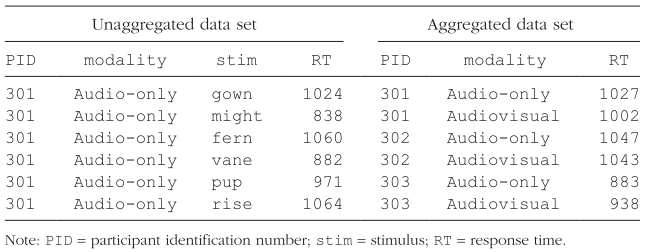
\includegraphics[scale=0.5]{Brown2021(1).png}
                \caption{Ejemplo de datos sin agregar.}
        \end{center}
\end{figure}

En un {\scshape Anova} normal habría solamente dos filas: una por cada modalidad, y cada fila contendría la media del tiempo de respuesta de todas las palabras presentadas a ese individuo.

{\scshape\bfseries Fixed and Random Effects}

Los modelos de efectos mixtos se llaman así debido a que modelan a la vez efectos fijos y aleatorios. Los fijos representan efectos a nivel de la población que deberían persistir entre experimentos ({\itshape e.g.,} promedio). Las condiciones suelen ser efectos fijos dado que se espera que operen en formas predecibles entre participantes e items. En este caso la modalidad será modelada como un efecto fijo.

Los efectos aleatorios modelan el nivel en el cual las tendencias medias varían entre niveles de un factor de agrupamiento (participantes o items). Son conglomerados de datos dependientes en los cuales las observaciones componentes vienen del mismo grupo de nivel superior (el mismo participante o item), y se incluyen en los modelos para dar cuenta de que la conducta de participantes o items individuales puede diferir de la tendencia media. Los efectos aleatorios son categóricos dado que son unidades discretas muestreadas de la población. Todo efecto que sea continuo tendrá que ser modelado como un efecto fijo. En este ejemplo se modela a participantes e items como efectos aleatorios dado que son muestreados al azar de sus poblaciones respectivas y se quiere dar cuenta de la variabilidad en ellas.

En los modelos mixtos el estimado del intercepto fijo representa el intercepto medio. Además, para cada participante e item se estima un intercepto aleatorio que les permite desviarse de esa media. Se asume que las desviaciones forman una distribución normal con media de cero y una varianza estimada por el modelo.




\end{document}
